\documentclass{standalone}
\usepackage{tikz}
\usetikzlibrary{patterns, positioning}

\begin{document}
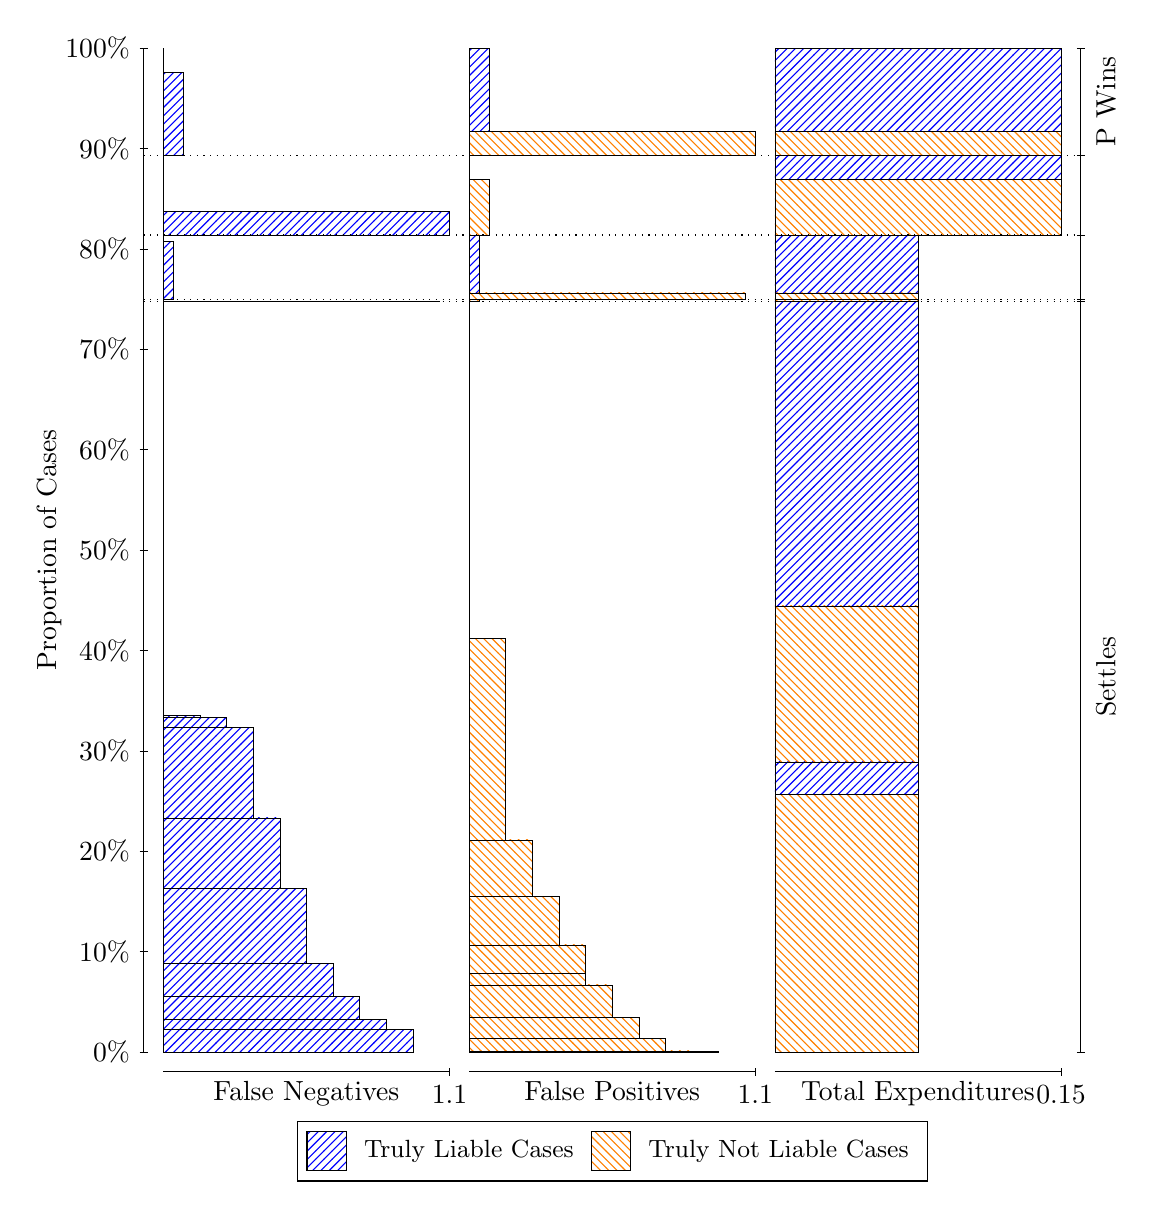
\begin{tikzpicture}
\draw[black, very thin] (1.5,1.75) -- (1.5,14.5);
\node[rotate=90, anchor=center] at (0.3, 8.125) {Proportion of Cases};
\draw[black, very thin] (1.45,1.75) -- (1.55,1.75);
\node[anchor=east] at (1.45, 1.75) {0\%};
\draw[black, very thin] (1.45,3.025) -- (1.55,3.025);
\node[anchor=east] at (1.45, 3.025) {10\%};
\draw[black, very thin] (1.45,4.3) -- (1.55,4.3);
\node[anchor=east] at (1.45, 4.3) {20\%};
\draw[black, very thin] (1.45,5.575) -- (1.55,5.575);
\node[anchor=east] at (1.45, 5.575) {30\%};
\draw[black, very thin] (1.45,6.85) -- (1.55,6.85);
\node[anchor=east] at (1.45, 6.85) {40\%};
\draw[black, very thin] (1.45,8.125) -- (1.55,8.125);
\node[anchor=east] at (1.45, 8.125) {50\%};
\draw[black, very thin] (1.45,9.4) -- (1.55,9.4);
\node[anchor=east] at (1.45, 9.4) {60\%};
\draw[black, very thin] (1.45,10.675) -- (1.55,10.675);
\node[anchor=east] at (1.45, 10.675) {70\%};
\draw[black, very thin] (1.45,11.95) -- (1.55,11.95);
\node[anchor=east] at (1.45, 11.95) {80\%};
\draw[black, very thin] (1.45,13.225) -- (1.55,13.225);
\node[anchor=east] at (1.45, 13.225) {90\%};
\draw[black, very thin] (1.45,14.5) -- (1.55,14.5);
\node[anchor=east] at (1.45, 14.5) {100\%};

\draw[black, very thin] (13.4,1.75) -- (13.4,14.5);
\draw[black, very thin] (13.35,1.75) -- (13.45,1.75);
\node[anchor=west] at (13.35, 1.75) {};
\draw[black, very thin] (13.35,11.28) -- (13.45,11.28);
\node[anchor=west] at (13.35, 11.28) {};
\draw[black, very thin] (13.35,11.308) -- (13.45,11.308);
\node[anchor=west] at (13.35, 11.308) {};
\draw[black, very thin] (13.35,12.125) -- (13.45,12.125);
\node[anchor=west] at (13.35, 12.125) {};
\draw[black, very thin] (13.35,13.135) -- (13.45,13.135);
\node[anchor=west] at (13.35, 13.135) {};
\draw[black, very thin] (13.35,14.5) -- (13.45,14.5);
\node[anchor=west] at (13.35, 14.5) {};

\draw[black, very thin, pattern color=blue, pattern=north east lines] (1.75,1.75) rectangle (4.9186,2.0388);
\draw[black, very thin, pattern color=blue, pattern=north east lines] (1.75,2.0388) rectangle (4.5806,2.1622);
\draw[black, very thin, pattern color=blue, pattern=north east lines] (1.75,2.1622) rectangle (4.2426,2.4513);
\draw[black, very thin, pattern color=blue, pattern=north east lines] (1.75,2.4513) rectangle (3.9047,2.8743);
\draw[black, very thin, pattern color=blue, pattern=north east lines] (1.75,2.8743) rectangle (3.5667,3.8228);
\draw[black, very thin, pattern color=blue, pattern=north east lines] (1.75,3.8228) rectangle (3.2287,4.7228);
\draw[black, very thin, pattern color=blue, pattern=north east lines] (1.75,4.7228) rectangle (2.8907,5.8756);
\draw[black, very thin, pattern color=blue, pattern=north east lines] (1.75,5.8756) rectangle (2.5527,5.9948);
\draw[black, very thin, pattern color=blue, pattern=north east lines] (1.75,5.9948) rectangle (2.2147,6.0273);
\draw[black, very thin, pattern color=orange, pattern=north west lines] (1.75,6.0273) rectangle (1.75,11.28);
\draw[black, very thin, pattern color=blue, pattern=north east lines] (1.75,11.28) rectangle (5.2566,11.282);
\draw[black, very thin, pattern color=orange, pattern=north west lines] (1.75,11.282) rectangle (1.75,11.308);
\draw[black, very thin, pattern color=blue, pattern=north east lines] (1.75,11.308) rectangle (1.8767,12.041);
\draw[black, very thin, pattern color=orange, pattern=north west lines] (1.75,12.041) rectangle (1.75,12.125);
\draw[black, very thin, pattern color=blue, pattern=north east lines] (1.75,12.125) rectangle (5.3833,12.429);
\draw[black, very thin, pattern color=orange, pattern=north west lines] (1.75,12.429) rectangle (1.75,13.135);
\draw[black, very thin, pattern color=blue, pattern=north east lines] (1.75,13.135) rectangle (2.0035,14.193);
\draw[black, very thin, pattern color=orange, pattern=north west lines] (1.75,14.193) rectangle (1.75,14.5);
\draw[black, very thin, pattern color=orange, pattern=north west lines] (5.6333,1.75) rectangle (8.8019,1.7526);
\draw[black, very thin, pattern color=orange, pattern=north west lines] (5.6333,1.7526) rectangle (8.464,1.7646);
\draw[black, very thin, pattern color=orange, pattern=north west lines] (5.6333,1.7646) rectangle (8.126,1.9273);
\draw[black, very thin, pattern color=orange, pattern=north west lines] (5.6333,1.9273) rectangle (7.788,2.1885);
\draw[black, very thin, pattern color=orange, pattern=north west lines] (5.6333,2.1885) rectangle (7.45,2.6015);
\draw[black, very thin, pattern color=orange, pattern=north west lines] (5.6333,2.6015) rectangle (7.112,2.7449);
\draw[black, very thin, pattern color=orange, pattern=north west lines] (5.6333,2.7449) rectangle (7.112,3.109);
\draw[black, very thin, pattern color=orange, pattern=north west lines] (5.6333,3.109) rectangle (6.774,3.7299);
\draw[black, very thin, pattern color=orange, pattern=north west lines] (5.6333,3.7299) rectangle (6.436,4.4436);
\draw[black, very thin, pattern color=orange, pattern=north west lines] (5.6333,4.4436) rectangle (6.0981,7.0026);
\draw[black, very thin, pattern color=blue, pattern=north east lines] (5.6333,7.0026) rectangle (5.6333,11.28);
\draw[black, very thin, pattern color=orange, pattern=north west lines] (5.6333,11.28) rectangle (5.7601,11.305);
\draw[black, very thin, pattern color=blue, pattern=north east lines] (5.6333,11.305) rectangle (5.6333,11.308);
\draw[black, very thin, pattern color=orange, pattern=north west lines] (5.6333,11.308) rectangle (9.1399,11.391);
\draw[black, very thin, pattern color=blue, pattern=north east lines] (5.6333,11.391) rectangle (5.7601,12.125);
\draw[black, very thin, pattern color=orange, pattern=north west lines] (5.6333,12.125) rectangle (5.8868,12.831);
\draw[black, very thin, pattern color=blue, pattern=north east lines] (5.6333,12.831) rectangle (5.6333,13.135);
\draw[black, very thin, pattern color=orange, pattern=north west lines] (5.6333,13.135) rectangle (9.2667,13.442);
\draw[black, very thin, pattern color=blue, pattern=north east lines] (5.6333,13.442) rectangle (5.8868,14.5);
\draw[black, very thin, pattern color=orange, pattern=north west lines] (9.5167,1.75) rectangle (11.333,5.0227);
\draw[black, very thin, pattern color=blue, pattern=north east lines] (9.5167,5.0227) rectangle (11.333,5.4349);
\draw[black, very thin, pattern color=orange, pattern=north west lines] (9.5167,5.4349) rectangle (11.333,7.4148);
\draw[black, very thin, pattern color=blue, pattern=north east lines] (9.5167,7.4148) rectangle (11.333,11.28);
\draw[black, very thin, pattern color=orange, pattern=north west lines] (9.5167,11.28) rectangle (11.333,11.305);
\draw[black, very thin, pattern color=blue, pattern=north east lines] (9.5167,11.305) rectangle (11.333,11.308);
\draw[black, very thin, pattern color=orange, pattern=north west lines] (9.5167,11.308) rectangle (11.333,11.391);
\draw[black, very thin, pattern color=blue, pattern=north east lines] (9.5167,11.391) rectangle (11.333,12.125);
\draw[black, very thin, pattern color=orange, pattern=north west lines] (9.5167,12.125) rectangle (13.15,12.831);
\draw[black, very thin, pattern color=blue, pattern=north east lines] (9.5167,12.831) rectangle (13.15,13.135);
\draw[black, very thin, pattern color=orange, pattern=north west lines] (9.5167,13.135) rectangle (13.15,13.442);
\draw[black, very thin, pattern color=blue, pattern=north east lines] (9.5167,13.442) rectangle (13.15,14.5);
\draw[black, dotted] (1.5,11.28) -- (13.4,11.28);
\draw[black, dotted] (1.5,11.308) -- (13.4,11.308);
\draw[black, dotted] (1.5,12.125) -- (13.4,12.125);
\draw[black, dotted] (1.5,13.135) -- (13.4,13.135);
\draw[black, very thin] (1.75,1.5) -- (5.3833,1.5);
\node[anchor=north] at (3.5667, 1.5) {False Negatives};
\draw[black, very thin] (5.3833,1.45) -- (5.3833,1.55);
\node[anchor=north] at (5.3833, 1.45) {1.1};

\draw[black, very thin] (5.6333,1.5) -- (9.2667,1.5);
\node[anchor=north] at (7.45, 1.5) {False Positives};
\draw[black, very thin] (9.2667,1.45) -- (9.2667,1.55);
\node[anchor=north] at (9.2667, 1.45) {1.1};

\draw[black, very thin] (9.5167,1.5) -- (13.15,1.5);
\node[anchor=north] at (11.333, 1.5) {Total Expenditures};
\draw[black, very thin] (13.15,1.45) -- (13.15,1.55);
\node[anchor=north] at (13.15, 1.45) {0.15};

\node[black, centered, rotate=90] at (13.72, 6.515) {Settles};



\node[black, centered, rotate=90] at (13.72, 13.818) {P Wins};

\draw (7.449999999999999,1.5) node[draw=none] (baseCoordinate) {};
\begin{scope}[align=center]
        \matrix[scale=0.5, draw=black, below=0.5cm of baseCoordinate, nodes={draw}, column sep=0.1cm]{
            \node[rectangle, draw, minimum width=0.5cm, minimum height=0.5cm, pattern=north east lines, pattern color=blue] {}; &
            \node[draw=none, font=\small] (B) {Truly Liable Cases}; &
            \node[rectangle, draw, minimum width=0.5cm, minimum height=0.5cm, pattern=north west lines, pattern color=orange] {}; &
            \node[draw=none, font=\small] (B) {Truly Not Liable Cases}; \\
            };
\end{scope}

\end{tikzpicture}
\end{document}